\section{Experiments}
\label{sec:experiments}

% Data sources: outputs/ablation_20261113/{tables,layered/v3w,robustness}
% and outputs/cleargrasp_ghost_20261116/summary.json.
% Split names: Oblique = synth_two_layer_v2, Clutter = v3, Wide = v3w.
% The current "Ours" and ablation values come from ab26_* runs with
% ResNet-50 single-view front-ends and ground-truth input masks in the standard evaluations.
% The "w/o DINOv3 features" rows currently report the ResNet-50 semantic-feature ablations.
% ClearGrasp's GHOST baseline is ghost_pred, which uses its own TransDINO masks.
% TODO: replace the provisional values with runs matching Section 3 and add the cross-view ablation.

\subsection{Setup}
\label{sec:exp-setup}

\paragraph{Data.}
We train on 7,776 views from scenes 60 and above of Oblique and Clutter (\cref{sec:data}), select checkpoints by masked PSNR on scenes 0--59 of Oblique, and test on scenes 0--59 of all three sets: Oblique (240 views), Clutter (240) and Wide (360).
Wide is used neither for training nor for checkpoint selection, so it is our main synthetic benchmark; full Oblique and Clutter tables are in the supplement.
For real images we use the 113 images of the ClearGrasp real-test split~\cite{cleargrasp}, which has ground truth for the front surface only and is never seen in training.
The input mask $\hat M$ is predicted by TransDINO~\cite{ghost} in all experiments, and one pair of front-ends serves all six backbones.
% TODO(data swap): confirm the number of views F_bg receives at test time (ClearGrasp images are single views).
$\mathcal{F}_{bg}$ receives all views of a synthetic test scene jointly; $\mathcal{F}_{sf}$ and the backbones run per view.

\paragraph{Baselines.}
\emph{Original} feeds the input $I$ to the backbone.
\emph{LaMa} feeds the inpainting $P$, which removes the glass together with what is seen through it (background layer only).
\emph{GHOST}~\cite{ghost} renders the object opaque and yields one layer, so we feed its output to the same backbones and compare on the surface layer.
\emph{Oracle} feeds the target image ($B^*$, $O^*$, or on ClearGrasp the photograph with the objects painted opaque) and bounds what an image front-end can achieve.
\Cref{fig:exp-qualitative} compares point clouds from Original, GHOST, and Phantom across four backbones.

\paragraph{Protocol and metrics.}
Each depth map is scaled by its median ratio to the ground truth over valid pixels outside the ground-truth mask $M$ dilated by 7\,px.
This uses ground-truth depth, so we evaluate relative geometry inside the mask, not metric scale.
Metrics are computed inside $M$ on pixels where all compared methods are valid: AbsRel (\%), RMSE, and $\delta_{1.05}$, the share of pixels with $\max(d/d^*, d^*/d) < 1.05$.
For layered results, the two predictions are first aligned as in \cref{sec:fusion} from predicted points only, and one ground-truth scale, computed on the background, is applied to both layers.
The aligned surface is z-buffer reprojected and can leave pixels empty, so we also report coverage and $\delta_{1.05}^{\mathrm{all}}$, which counts empty pixels as failures.
Layer-order error is the share of mask pixels where the surface lies behind the background.
An alignment fails when the median residual on the held-out correspondences exceeds 4\% of the median point distance or, for RANSAC, when fewer than 30\% of the pairs are inliers.

\paragraph{Seeds and statistics.}
The main front-ends are trained with three seeds; we report mean$\pm$std for VGGT, $\pi^3$ and DA-V2 and seed~0 elsewhere.
A difference is significant when the 95\% CI of a paired bootstrap over scenes excludes zero for every available seed.

\providecommand{\sd}[1]{{\scriptsize$\pm$#1}}
\newcommand{\tbgray}[1]{\textcolor{gray}{#1}}
\newcommand{\tbgood}[2]{\expheat{ExpGood!#1!ExpMid}{#2}}
\newcommand{\tbpoor}[2]{\expheat{ExpMid!#1!ExpPoor}{#2}}

\begin{table*}[t]
\centering
\footnotesize
\renewcommand{\arraystretch}{1.0}
\setlength{\tabcolsep}{2pt}
\begin{tabular*}{\textwidth}{@{}l@{\extracolsep{\fill}}ccccccccccc@{}}
\toprule
 & \multicolumn{4}{c}{\emph{Background: full mask}} & \multicolumn{4}{c}{\emph{Background: through region}} & \multicolumn{3}{c}{\emph{Front surface}} \\
\cmidrule(lr){2-5}\cmidrule(lr){6-9}\cmidrule(lr){10-12}
Backbone & Original & LaMa & \textbf{Ours} & \tbgray{Oracle} & Original & LaMa & \textbf{Ours} & \tbgray{Oracle} & Original & \textbf{Ours} & \tbgray{Oracle} \\
\midrule
VGGT~\cite{vggt} & \tbpoor{0}{13.55} & \tbgood{93}{\underline{1.96}} & \tbgood{100}{\textbf{1.51\sd{.06}}} & \tbgray{0.89} & \tbpoor{0}{7.72} & \tbpoor{41}{\underline{6.70}} & \tbgood{100}{\textbf{2.73\sd{.08}}} & \tbgray{1.62} & \tbpoor{0}{\underline{9.09}} & \tbgood{100}{\textbf{4.25\sd{.32}}} & \tbgray{2.55} \\
$\pi^3$~\cite{pi3} & \tbpoor{0}{12.95} & \tbgood{99}{\underline{1.95}} & \tbgood{100}{\textbf{1.91\sd{.05}}} & \tbgray{0.76} & \tbpoor{0}{9.60} & \tbpoor{70}{\underline{7.18}} & \tbgood{100}{\textbf{2.66\sd{.12}}} & \tbgray{1.55} & \tbpoor{0}{\underline{7.89}} & \tbgood{100}{\textbf{3.13\sd{.22}}} & \tbgray{1.87} \\
DA-V2~\cite{dav2} & \tbpoor{0}{22.45} & \tbgood{92}{\underline{2.52}} & \tbgood{100}{\textbf{1.70\sd{.01}}} & \tbgray{1.40} & \tbpoor{0}{11.92} & \tbgood{1}{\underline{7.81}} & \tbgood{100}{\textbf{3.81\sd{.02}}} & \tbgray{2.37} & \tbpoor{0}{\underline{24.20}} & \tbgood{100}{\textbf{4.37\sd{.13}}} & \tbgray{3.62} \\
DA3~\cite{da3} & \tbpoor{0}{11.16} & \tbgood{84}{\underline{2.01}} & \tbgood{100}{\textbf{1.24}} & \tbgray{0.89} & \tbpoor{8}{\underline{7.11}} & \tbpoor{0}{7.27} & \tbgood{100}{\textbf{3.08}} & \tbgray{2.26} & \tbpoor{0}{\underline{9.81}} & \tbgood{100}{\textbf{3.69}} & \tbgray{2.87} \\
MoGe-2~\cite{moge2} & \tbpoor{0}{12.01} & \tbgood{100}{\textbf{1.90}} & \tbgood{70}{\underline{3.41}} & \tbgray{0.92} & \tbpoor{0}{9.24} & \tbpoor{69}{\underline{7.34}} & \tbgood{100}{\textbf{3.75}} & \tbgray{2.13} & \tbpoor{0}{\underline{7.54}} & \tbgood{100}{\textbf{4.10}} & \tbgray{2.92} \\
MoGe-3~\cite{moge3} & \tbpoor{0}{12.19} & \tbgood{100}{\textbf{2.05}} & \tbgood{63}{\underline{3.95}} & \tbgray{1.02} & \tbpoor{0}{9.50} & \tbpoor{86}{\underline{7.23}} & \tbgood{100}{\textbf{4.22}} & \tbgray{2.16} & \tbpoor{0}{\underline{7.21}} & \tbgood{100}{\textbf{4.22}} & \tbgray{2.87} \\
\bottomrule
\end{tabular*}
\caption{\textbf{Layered depth on Wide} (AbsRel \%, $\downarrow$; 360 views never used in training). Through denotes background objects seen through glass. In all tables, green/red indicate better/worse results within each comparison group; bold/underlined mark best/second best. Gray Oracle references are excluded.}
\label{tab:exp-synthetic}
\end{table*}

\begin{figure*}[t]
\centering
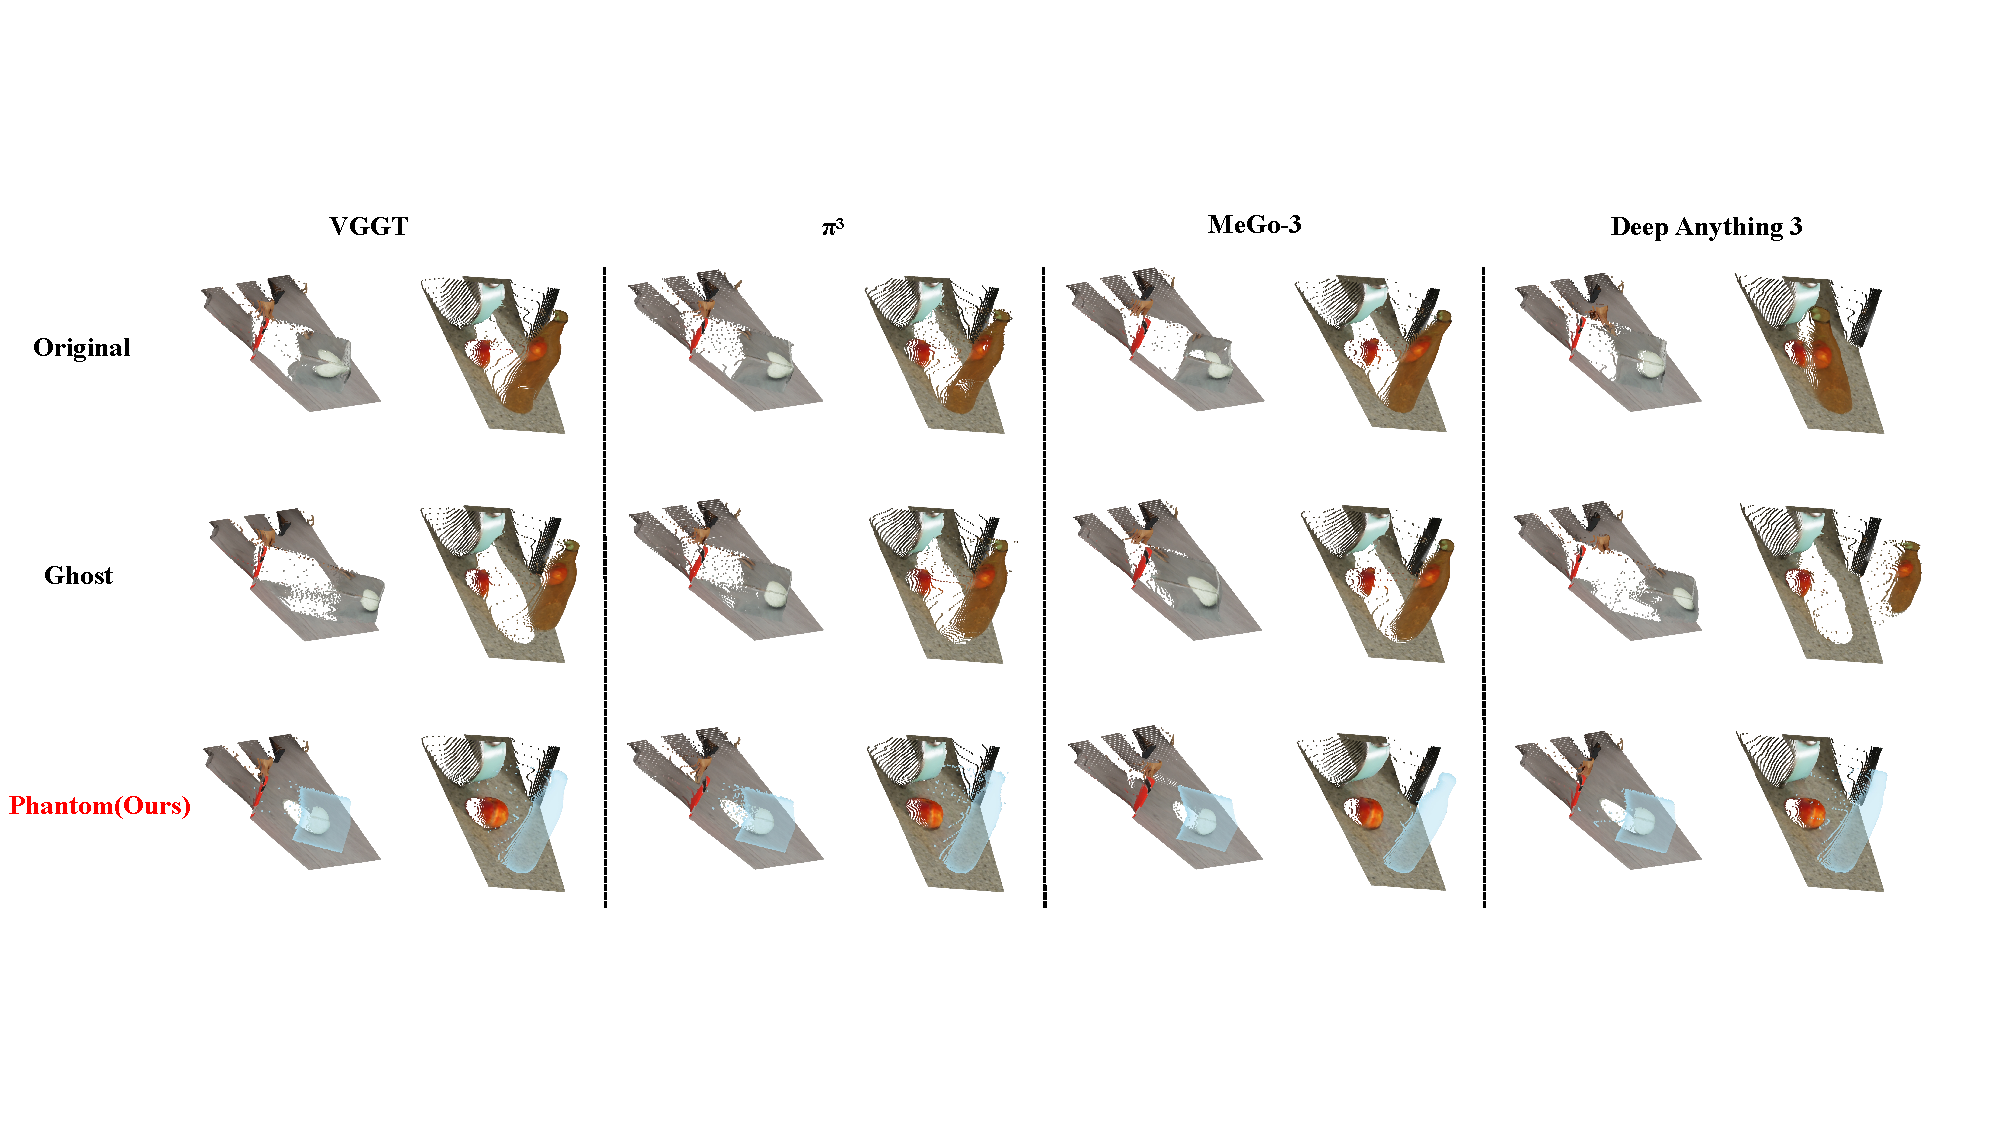
\includegraphics[pagebox=cropbox,width=\textwidth]{fig/qualitative_comparison.pdf}
\caption{\textbf{Qualitative point-cloud comparison.}
Each column group shows two example views for VGGT, $\pi^3$, MoGe-3, or Depth Anything 3.
From top to bottom, the rows show the original backbone, GHOST, and Phantom with the same backbone.}
\label{fig:exp-qualitative}
\end{figure*}

\subsection{Synthetic Layered Scenes}
\label{sec:exp-synthetic}

\Cref{tab:exp-synthetic} reports both layers on Wide.
With the original image, every backbone has 11--22\% AbsRel on the background and 7--24\% on the front surface, because it predicts one depth that mixes the two layers.
Phantom lowers the surface error on all six backbones, by 41\% (MoGe-3) to 82\% (DA-V2), and the background error to 1.2--4.0\%.

The through region shows what the background front-end adds over inpainting.
LaMa replaces the glass with a plausible table, which is correct for most mask pixels, so on the full mask it reaches 1.9--2.5\%.
Behind the glass, however, it hallucinates over the objects the camera actually sees, and its through-region error stays at 6.7--7.8\%, close to the Original.
Phantom keeps this content and reduces the through-region error to 2.7--4.2\% on every backbone.
On the full mask Phantom beats LaMa on four backbones but not on MoGe-2 and MoGe-3 (3.41 \vs 1.90 and 3.95 \vs 2.05).
We have not identified the cause; one possibility is that $\mathcal{L}_{\mathrm{geo}}$ uses a DA-V2 network whose preferences transfer poorly to MoGe.
Oblique and Clutter show the same pattern, including a slightly worse full-mask background than LaMa for $\pi^3$ (supplement).

\begin{table}[t]
\centering
\footnotesize
\renewcommand{\arraystretch}{1.0}
\setlength{\tabcolsep}{2pt}
\begin{tabular*}{\columnwidth}{@{}l@{\extracolsep{\fill}}ccccccc@{}}
\toprule
 & \multicolumn{4}{c}{AbsRel (\%, $\downarrow$)} & \multicolumn{3}{c}{RMSE (mm, $\downarrow$)} \\
\cmidrule(lr){2-5}\cmidrule(lr){6-8}
Backbone & Orig. & GHOST & \textbf{Ours} & \tbgray{Oracle} & Orig. & GHOST & \textbf{Ours} \\
\midrule
VGGT & \tbpoor{0}{7.84} & \tbgood{54}{\underline{4.00}} & \tbgood{100}{\textbf{2.86}} & \tbgray{2.35} & \tbpoor{0}{46.4} & \tbgood{46}{\underline{25.7}} & \tbgood{100}{\textbf{18.0}} \\
$\pi^3$ & \tbpoor{0}{6.71} & \tbgood{39}{\underline{4.14}} & \tbgood{100}{\textbf{3.02}} & \tbgray{1.98} & \tbpoor{0}{41.0} & \tbgood{37}{\underline{26.1}} & \tbgood{100}{\textbf{19.3}} \\
DA-V2 & \tbgood{56}{\underline{3.71}} & \tbpoor{0}{4.94} & \tbgood{100}{\textbf{3.36}} & \tbgray{2.81} & \tbgood{72}{\underline{23.4}} & \tbpoor{0}{30.9} & \tbgood{100}{\textbf{22.2}} \\
DA3 & \tbpoor{0}{4.79} & \tbpoor{1}{\underline{4.78}} & \tbgood{100}{\textbf{3.44}} & \tbgray{1.89} & \tbpoor{46}{\underline{29.0}} & \tbpoor{0}{31.1} & \tbgood{100}{\textbf{21.9}} \\
MoGe-2 & \tbpoor{0}{10.09} & \tbgood{35}{\underline{5.92}} & \tbgood{100}{\textbf{3.90}} & \tbgray{1.89} & \tbpoor{0}{57.1} & \tbgood{27}{\underline{35.9}} & \tbgood{100}{\textbf{23.8}} \\
MoGe-3 & \tbpoor{0}{9.80} & \tbgood{43}{\underline{5.20}} & \tbgood{100}{\textbf{3.38}} & \tbgray{1.62} & \tbpoor{0}{55.2} & \tbgood{38}{\underline{31.8}} & \tbgood{100}{\textbf{21.2}} \\
\midrule
Mean & \tbpoor{0}{7.16} & \tbgood{22}{\underline{4.83}} & \tbgood{100}{\textbf{3.33}} & \tbgray{2.09} & \tbpoor{0}{42.0} & \tbgood{13}{\underline{30.2}} & \tbgood{100}{\textbf{21.1}} \\
\bottomrule
\end{tabular*}
\caption{\textbf{Front-surface depth on ClearGrasp real-test} (113 images, inside the ground-truth mask). GHOST and Ours receive the same TransDINO masks. Ours is trained on synthetic data only; GHOST uses its released weights. Colors compare methods within each backbone and metric.}
\label{tab:exp-real}
\end{table}

\subsection{Real Transparent Objects}
\label{sec:exp-real}

\Cref{tab:exp-real} evaluates the front surface on ClearGrasp.
Phantom has the lowest error of the non-Oracle inputs on all six backbones and lowers the mean AbsRel from 7.16\% to 3.33\%, compared with 4.83\% for GHOST.
The gain is largest where the original prediction fails most (MoGe-2: 10.09 to 3.90\%); DA-V2, which already handles these images fairly well, improves from 3.71 to 3.36\%.
GHOST improves four backbones but is worse than Original on DA-V2 (4.94\%) and on par with it on DA3 (4.78\%).
Both methods inherit the errors of TransDINO, whose masks reach a mean IoU of 0.74 on these images (median 0.88; 23 of 113 below 0.5).
The remaining gap to the Oracle, 1.2 points on average, is the room left for a better surface front-end.

\begin{table}[t]
\centering
\footnotesize
\renewcommand{\arraystretch}{1.0}
\setlength{\tabcolsep}{3pt}
\begin{tabular*}{\columnwidth}{@{}l@{\extracolsep{\fill}}ccccc@{}}
\toprule
 & \multicolumn{2}{c}{AbsRel (\%) $\downarrow$} & \multicolumn{2}{c}{Order (\%) $\downarrow$} & $\delta^{\mathrm{all}}_{1.05}\uparrow$ \\
\cmidrule(lr){2-3}\cmidrule(lr){4-5}
Front-ends & Backgr. & Surface & VGGT & 6-mean &  \\
\midrule
None (Original) & \expheat{ExpMid!0!ExpPoor}{\underline{13.55}} & \expheat{ExpMid!0!ExpPoor}{9.09} & \textcolor{gray}{0.00$^\ast$} & \textcolor{gray}{0.00$^\ast$} & \expheat{ExpMid!13!ExpPoor}{52.7} \\
$\mathcal{F}_{bg}$ only & \expheat{ExpGood!100!ExpMid}{\textbf{1.55}} & \expheat{ExpMid!2!ExpPoor}{9.05} & \expheat{ExpGood!84!ExpMid}{\underline{2.41}} & \expheat{ExpGood!22!ExpMid}{\underline{7.84}} & \expheat{ExpMid!0!ExpPoor}{51.1} \\
$\mathcal{F}_{sf}$ only & \expheat{ExpMid!0!ExpPoor}{\underline{13.55}} & \expheat{ExpGood!99!ExpMid}{\underline{4.62}} & \expheat{ExpMid!0!ExpPoor}{23.34} & \expheat{ExpMid!0!ExpPoor}{17.89} & \expheat{ExpGood!100!ExpMid}{\textbf{76.7}} \\
\textbf{Both (Ours)} & \expheat{ExpGood!100!ExpMid}{\textbf{1.55}} & \expheat{ExpGood!100!ExpMid}{\textbf{4.60}} & \expheat{ExpGood!100!ExpMid}{\textbf{0.60}} & \expheat{ExpGood!100!ExpMid}{\textbf{1.38}} & \expheat{ExpGood!96!ExpMid}{\underline{76.2}} \\
\bottomrule
\end{tabular*}
\caption{\textbf{Branch combination} on Wide (VGGT, seed~0). A disabled branch uses the original image. Order denotes layer-order error (VGGT and six-backbone mean). $^\ast$Trivial zeros from identical predictions are excluded from ranking and coloring.}
\label{tab:exp-branches}
\end{table}

\subsection{Ablation Studies}
\label{sec:exp-analysis}

\paragraph{Both front-ends are needed.}
\Cref{tab:exp-branches} enables the front-ends one at a time.
Each front-end improves only its own layer.
With the surface front-end alone, the background is still the mixed original prediction, which lies in front of the restored surface at 23\% of the mask pixels for VGGT.
With both front-ends the layer-order error drops to 0.60\% for VGGT and to 1.38\% on average over the six backbones.
Adding the background front-end leaves the surface accuracy nearly unchanged (AbsRel 4.62 \vs 4.60, $\delta^{\mathrm{all}}_{1.05}$ 76.7 \vs 76.2), so the order improvement does not come at the cost of the surface.

\paragraph{Alignment.}
Averaged over the six backbones on Wide, fusing the two predictions without alignment fails in 44\% of the views (up to 86\% for MoGe-3) and gives 9.45\% surface AbsRel, because independent predictions differ in scale.
A single scale already removes most of the discrepancy (4.07\%, 0.05\% failures), and a least-squares Sim(3) fails in up to 5\% of the views of a backbone.
RANSAC Sim(3) has no failures and gives 4.16\% AbsRel; we use it by default, and scale-only alignment is a simpler alternative of similar accuracy (supplement).

\begin{table}[t]
\centering
\footnotesize
\renewcommand{\arraystretch}{1.0}
\setlength{\tabcolsep}{3pt}
\begin{tabular*}{\columnwidth}{@{}c@{\hspace{4pt}}l@{\extracolsep{\fill}}cccc@{}}
\toprule
& Variant & VGGT $\downarrow$ & $\pi^3\downarrow$ & DA-V2 $\downarrow$ & PSNR $\uparrow$ \\
\midrule
\multirow{9}{*}{\rotatebox{90}{$\mathcal{F}_{bg}$}}
 & w/o LaMa prior & \expheat{ExpMid!0!ExpPoor}{2.77\sd{.13}$^\dagger$} & \expheat{ExpMid!0!ExpPoor}{3.69\sd{.57}$^\dagger$} & \expheat{ExpGood!30!ExpMid}{1.78\sd{.01}} & \expheat{ExpMid!96!ExpPoor}{24.08\sd{.04}} \\
 & Prior as input only & \expheat{ExpGood!22!ExpMid}{2.00$^\dagger$} & \expheat{ExpGood!3!ExpMid}{2.69$^\dagger$} & \expheat{ExpGood!100!ExpMid}{\textbf{1.70}} & \expheat{ExpGood!73!ExpMid}{24.46} \\
 & Fixed 0.5/0.5 fusion & \expheat{ExpGood!48!ExpMid}{1.84$^\dagger$} & \expheat{ExpGood!9!ExpMid}{2.63$^\dagger$} & \expheat{ExpGood!48!ExpMid}{1.76$^\dagger$} & \expheat{ExpMid!96!ExpPoor}{24.08$^\dagger$} \\
 & w/o LPIPS & \expheat{ExpMid!65!ExpPoor}{2.36$^\dagger$} & \expheat{ExpMid!88!ExpPoor}{2.84$^\dagger$} & \expheat{ExpMid!0!ExpPoor}{1.93$^\dagger$} & \expheat{ExpGood!45!ExpMid}{24.32$^\dagger$} \\
 & w/o detail CNN & \expheat{ExpGood!86!ExpMid}{1.60\sd{.07}} & \expheat{ExpGood!60!ExpMid}{2.14\sd{.07}} & \expheat{ExpGood!74!ExpMid}{1.73\sd{.01}} & \expheat{ExpMid!51!ExpPoor}{23.86\sd{.06}$^\dagger$} \\
 & w/o DINOv3 & \expheat{ExpGood!78!ExpMid}{1.65} & \expheat{ExpGood!58!ExpMid}{2.16} & \expheat{ExpMid!43!ExpPoor}{1.88$^\dagger$} & \expheat{ExpMid!0!ExpPoor}{23.61$^\dagger$} \\
 & w/o $\mathcal{L}_{\mathrm{geo}}$ & \expheat{ExpGood!92!ExpMid}{1.56\sd{.01}} & \expheat{ExpGood!75!ExpMid}{1.99\sd{.02}} & \expheat{ExpGood!91!ExpMid}{\underline{1.71\sd{.03}}} & \expheat{ExpGood!100!ExpMid}{\textbf{24.59\sd{.04}}} \\
 & w/o $T$ weighting & \expheat{ExpGood!98!ExpMid}{\underline{1.52\sd{.04}}} & \expheat{ExpGood!100!ExpMid}{\textbf{1.75\sd{.11}}} & \expheat{ExpGood!100!ExpMid}{\textbf{1.70\sd{.02}}} & \expheat{ExpGood!86!ExpMid}{\underline{24.52\sd{.02}}} \\
 & \textbf{Full (Ours)} & \expheat{ExpGood!100!ExpMid}{\textbf{1.51\sd{.06}}} & \expheat{ExpGood!84!ExpMid}{\underline{1.91\sd{.05}}} & \expheat{ExpGood!100!ExpMid}{\textbf{1.70\sd{.01}}} & \expheat{ExpGood!73!ExpMid}{24.46\sd{.09}} \\
\midrule
\multirow{5}{*}{\rotatebox{90}{$\mathcal{F}_{sf}$}}
 & w/o $\mathcal{L}_{\mathrm{geo}}$ & \expheat{ExpMid!80!ExpPoor}{4.67\sd{.13}} & \expheat{ExpGood!42!ExpMid}{\underline{3.22\sd{.25}}} & \expheat{ExpGood!83!ExpMid}{4.60\sd{.31}} & \expheat{ExpGood!1!ExpMid}{19.03\sd{.10}} \\
 & w/o detail CNN & \expheat{ExpGood!9!ExpMid}{4.57\sd{.16}} & \expheat{ExpMid!0!ExpPoor}{3.44\sd{.31}} & \expheat{ExpGood!91!ExpMid}{\underline{4.49\sd{.11}}} & \expheat{ExpGood!100!ExpMid}{\textbf{19.53\sd{.37}}} \\
 & w/o DINOv3 & \expheat{ExpMid!0!ExpPoor}{4.95} & \expheat{ExpMid!0!ExpPoor}{3.44} & \expheat{ExpGood!57!ExpMid}{4.94} & \expheat{ExpMid!59!ExpPoor}{18.82} \\
 & w/o LPIPS & \expheat{ExpGood!63!ExpMid}{\underline{4.38}} & \expheat{ExpMid!77!ExpPoor}{3.32} & \expheat{ExpMid!0!ExpPoor}{7.03$^\dagger$} & \expheat{ExpMid!0!ExpPoor}{18.52$^\dagger$} \\
 & \textbf{Full (Ours)} & \expheat{ExpGood!100!ExpMid}{\textbf{4.25\sd{.32}}} & \expheat{ExpGood!100!ExpMid}{\textbf{3.13\sd{.22}}} & \expheat{ExpGood!100!ExpMid}{\textbf{4.37\sd{.13}}} & \expheat{ExpGood!17!ExpMid}{\underline{19.11\sd{.12}}} \\
\bottomrule
\end{tabular*}
\caption{\textbf{Component ablation} on Wide (AbsRel \%, and masked PSNR in dB). $^\dagger$: the paired scene-bootstrap 95\% CI of the difference to the full model excludes zero for every seed. Std uses three seeds; other rows use seed~0. Colors compare variants within each front-end and metric.}
\label{tab:exp-ablation}
\end{table}

\paragraph{Components.}
\Cref{tab:exp-ablation} removes one component at a time.
For the background, the LaMa prior and the learned fusion matter most.
Without the prior, VGGT's error rises from 1.51 to 2.77\%; giving the prior to the network only as an input (2.00\%) or mixing it with fixed weights (1.84\%) recovers part of the gap.
Removing LPIPS hurts every backbone.
The detail CNN and the DINOv3 features mainly improve the image (PSNR $-0.60$ and $-0.85$\,dB without them), with smaller changes in depth.
For the surface, every removal increases the mean error, but most differences are not significant in all seeds.
$\mathcal{L}_{\mathrm{geo}}$ reduces the VGGT surface error from 4.67 to 4.25\% on average, with a significant difference in two of three seeds, and has no measurable effect on the background.
Two non-default settings are better on Wide (geometry weight 1.0 for the background, no auxiliary terms for the surface); we fixed the defaults before the ablation and report these variants in the supplement.

\paragraph{Mask errors.}
Because Phantom edits only the masked region, a mask that misses part of the object leaves that part unchanged.
We perturb the input mask, recompute the LaMa prior, and keep the evaluation mask fixed (seed~0, VGGT / $\pi^3$ / DA-V2).
Dilating the mask by 3 or 7\,px does not hurt (background 1.1--2.0\%, surface 2.9--4.8\%, close to the unperturbed values).
A (3, 3)\,px shift raises the background error to 7.2--10.3\%, and a 3\,px erosion to 13.1--20.3\%, the level of the original image, with the VGGT surface error rising to 9.03\%.
Over-segmentation is therefore much safer than under-segmentation, and the mask predictor should be biased towards larger masks.

\subsection{Limitations}
\label{sec:exp-limitations}

Phantom depends on the mask: pixels it misses are not edited (\cref{sec:exp-analysis}).
There is no real benchmark with ground truth for both layers, so the hidden background is evaluated on synthetic data only, real images test only the front surface, and all depths are evaluated up to a ground-truth scale.
Only the background front-end uses several views, and its attention has no camera geometry; the backbone, the alignment and the fusion run per view, so the layered clouds of different views are not merged into one scene.
On MoGe-2 and MoGe-3 the restored background still trails LaMa, so the front-ends do not yet transfer equally well to every backbone.
